% Created 2016-01-29 Vi 17:49
\documentclass[presentation]{beamer}
\usepackage[utf8]{inputenc}
\usepackage[T1]{fontenc}
\usepackage{fixltx2e}
\usepackage{graphicx}
\usepackage{longtable}
\usepackage{float}
\usepackage{wrapfig}
\usepackage{rotating}
\usepackage[normalem]{ulem}
\usepackage{amsmath}
\usepackage{textcomp}
\usepackage{marvosym}
\usepackage{wasysym}
\usepackage{amssymb}
\usepackage{hyperref}
\tolerance=1000
\usetheme{default}
\author{mihai}
\date{\today}
\title{1}
\hypersetup{
  pdfkeywords={},
  pdfsubject={},
  pdfcreator={Emacs 24.5.1 (Org mode 8.2.10)}}
\begin{document}

\maketitle
\begin{frame}{Outline}
\tableofcontents
\end{frame}

\begin{frame}[label=sec-1]{1. Ce sunt circuitele „serie” şi „paralel”}
Circuitele formate dintr-o singură baterie şi o singură rezistenţă sunt
foarte uşor de analizat, dar nu sunt foarte des întâlnite în practică.
De obicei circuitele conţin mai mult de două componente conectate între
ele

Există două modalităţi de bază în care putem conecta mai mult de două
componente într-un circuit: \emph{serie} şi \emph{paralel}. Mai jos e un exemplu
de circuit serie:

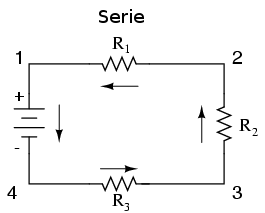
\includegraphics[width=.9\linewidth]{../poze/00082.png}

În acest circuit avem 3 rezistori (R$_{\text{1}}$,R$_{\text{2}}$ şi R$_{\text{3}}$) conectaţi
într-un singur lanţ de la un terminal al bateriei la celălalt.
Caracteristica principală a unui circuit serie este existenţa unei
singure căi pentru curgerea electronilor.

Să ne uităm acum şi la celălalt tip de circuit, cel paralel:

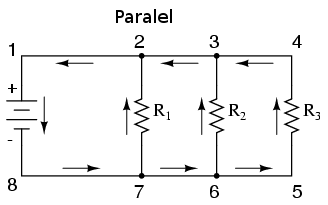
\includegraphics[width=.9\linewidth]{../poze/00083.png}

Şi în acest caz avem tot 3 rezistori, dar de data această există mai
multe căi pentru curgerea electronilor. Există o cale de la 8 la 7, 2, 1
şi înapoi la 8. Mai exista una de la 8 la 7, 6, 3, 2, 1 şi înapoi la 8.
Şi mai există o a treia cale de la 8 la 7, 6, 5, 4, 3, 2, 1 şi înapoi la
\begin{enumerate}
\item Fiecare cale individuală (prin R$_{\text{1}}$,R$_{\text{2}}$ şi R$_{\text{3}}$) poartă denumirea
\end{enumerate}
de \emph{ramură}

Caracteristica definitorie pentru un circuit paralel este faptul că
toate componentele sunt conectate electric între aceleaşi seturi de
puncte. În circuitul de mai sus, punctele 1, 2, 3 şi 4 sunt toate comune
din punct de vedere electric. La fel şi punctele 8, 7, 6 şi 5. Toate
rezistoarele, precum şi bateria, sunt conectate între aceste două
puncte.

Desigur, complexitatea nu se opreşte nici la circuite serie sau paralel!
Putem avea de asemenea circuite ce sunt o combinaţie dintre acestea
două:

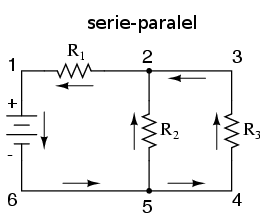
\includegraphics[width=.9\linewidth]{../poze/00084.png}

În acest circuit, avem două ramuri prin care electroni pot să circule:
una de la 6 la 5, 2, 1 şi înapoi la 6, iar altă ramură de la 6 la 5, 4,
3, 2, 1 şi înapoi la 6. Observaţi cum ambele drumuri trec prin R$_{\text{1}}$ (de
la punctul 2 spre punctul 1). În această configuraţie, spunem că R$_{\text{1}}$
şi R$_{\text{2}}$ sunt paralele între ele, în timp ce R$_{\text{1}}$ este în serie cu
combinaţia paralelă R$_{\text{1}}$ şi R$_{\text{2}}$.

Idea de bază într-o conexiune serie este conectarea componentelor de la
un capăt la altul într-o linie dreaptă:

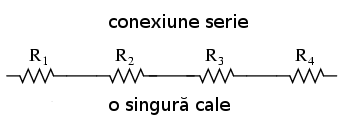
\includegraphics[width=.9\linewidth]{../poze/00085.png}

Idea de bază într-o conexiune paralel, pe de altă parte, este că toate
componentele sunt conectate între la aceleaşi capete. Într-un circuit
pur paralel, nu există niciodată mai mult de două puncte comune,
indiferent de numărul componentelor din circuit conectate. Există mai
mult de o singură cale pentru deplasarea electronilor, dar o singură
cădere de tensiune asupra tuturor componentelor"

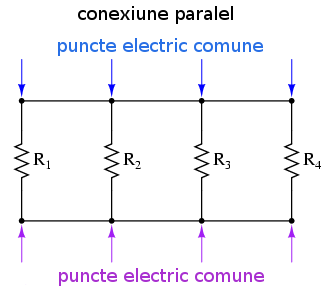
\includegraphics[width=.9\linewidth]{../poze/00086.png}

Cele două tipuri de configuraţii, serie şi paralel, prezintă proprietăţi
electrice total diferite.

Sumar:

\begin{itemize}
\item Într-un circuit serie, toate componentele sunt conectate unul în
continuarea celuilalt, formând o singură cale pentru curgerea
electronilor.
\item Într-un circuit paralel, toate componentele sunt conectate la acelaşi
capăt, formând exact un set de două puncte electric comune.
\item O „ramură” într-un circuit paralel este o cale pentru curgerea
curentului formată din cel puţin o sarcină (rezistenţă) din circuit.
\item Legea lui Ohm: E = IR; I = E/R; R = E/I
\end{itemize}
\end{frame}
% Emacs 24.5.1 (Org mode 8.2.10)
\end{document}
